\documentclass[11pt]{article}
\usepackage{graphicx}
\usepackage{amsmath}
\usepackage{amsfonts}
\usepackage{amssymb}
\usepackage{setspace}
\usepackage{booktabs}
\usepackage{cancel}
\usepackage{float}
\usepackage{sectsty}

\usepackage[T1]{fontenc}
\usepackage{textcomp}
\usepackage{listings}
\lstset{upquote=true}

\usepackage[most]{tcolorbox}
\usepackage{algorithm2e}

%setting page size
\setlength{\oddsidemargin}{0.0in}
\setlength{\textwidth}{6.5in}
\setlength{\topmargin}{-0.5in}
\setlength{\footskip}{0.30in}
\setlength{\textheight}{9.0in}
\setlength{\headheight}{0.2in}
\setlength{\headsep}{0.3in}
%
\newcommand{\tet}{\texttt}


\newcommand{\argmin}{\mathop{\mathrm{arg\,min}}}

\newcommand{\commentJK}[1]{\begin{center}\begin{minipage}{0.8\textwidth}\it\color{cyan}Comment:  #1\end{minipage}\end{center}}

\begin{document}

\title{Thresholding Method for simulating the alternate KWC model\\ Code User Manual}
\author{Jaekwang Kim, Matt Jacobs, Nikhil Chandra Admal} 

\maketitle 
\sectionfont{\fontsize{14}{14}\selectfont}

\normalsize

\section{Introduction}

This is the user manual for illustrating details of 
the numerical scheme suggested in the white paper.
A \texttt{C++} based software is developed
to simulate the kinetics of grain growth described by   
defined by KWC (Kobayashi--Warren--Carter) model~\cite{KWC:1998,KWC:2001,KWC:2003}

%Begin Algorithm Alternate KWC simulation
\begin{algorithm}
    \setstretch{1.1}\small
    \SetKwInOut{Input}{Input} % For compile
    \SetKwInOut{Output}{Output} % For compile
    \Input{System size $N$, parameter $\epsilon,\xi$ and  an initial grain configuration $\theta^{0}$}
    \Output{Time evolution of the alternate KWC model} 
    
    Initialize Grains $\theta^{0}$ on domain $\Omega$\\
    \While{ t $<$ T} {
    Compute grain boundary energy $\mathcal{J} \big( [\![ \theta ]\!] \big)$\\
    
    \hfill\linebreak     
    \CommentSty{Execute Primal-dual algorithm}\\
    
     \While{$\mathrm{max}(\eta^{n+1}-\eta^{n})< tol$}
    {
    Update $\eta^{n+1}$ using $\psi^{n}$  
    Update $\psi^{n+1}$ using $\eta^{n+1}$  
    }
     
    \hfill\linebreak    
    \CommentSty{Execute thresholding algorithm}\\
    
    Identify interior regions of grains $I_p$ 
    
    \quad\quad  \CommentSty{Execute Fast Marching}\\
    \quad\quad Allow each grain $I_p$ to grow with speed $1/(1-\eta)^2$\\
    \quad\quad Threshold $\theta(x), x\in \Omega-I$ to that of a interior grain arrives at earliest  
     
    \hfill\linebreak
    Compute free energy $\mathcal{W}_{\mathrm{kwc}}(\eta,\theta)$\\

    } %End of time (t<T) while
    \caption{Suggested algorithms for the alternative KWC simulation}
    \label{algorithm:KWC}
\end{algorithm}
%% End algorithm 


In this model, the material free energy density $\mathcal{W}$ 
is defined by two field variable: the order-phase parameter $\eta$ 
and the orientation-phase parameter $\theta$. 
The free energy of the alternate KWC is 
\begin{equation}
\mathcal{W}[\eta,\theta] = \int
\left[ \frac{(1-\eta)^2}{2 \epsilon} + \frac{\epsilon}{2}|\nabla \phi|^2
+sg(\eta) \mathcal{J}\big( [\![\theta ]\!]\big) \delta(x-x_0) 
\right]\; dV.
\label{eqn:alternateKWC}
\end{equation}
The code solves the KWC gradient flow 
by iteratively solving the following optimization problems:
\begin{equation}
\eta^{k+1}=\argmin_\eta \mathcal{W}[\eta, \theta^{k}] 
\end{equation}
\begin{equation}
\theta^{k+1}=\argmin_\theta  \mathcal{W}[\eta^{k+1}, \theta] 
\end{equation}
To solve the $\eta$-sub problem, 
the code uses the Primal-dual algorithm~\cite{Chambolle:2011,Jacobs:2019}.
For second, the $\theta$-sub problem, 
we use thresholding dynamics. 

The developed code has a modularized structure. 
A user-program can be executed by through a driver file 
(we suggest a \texttt{.cpp} format) 
referring necessary C++ functions and classes from different header files,
which are categorized by its task.
Each function and class can be replaced by a user-defined form, 
as long as the input \& output formatting is consistent. 
The list of header files is summarized in Table 1. 
and the flow chart of algorithm is attached in Figure~\ref{Fig:flow_chart}\\

\begin{table}[b]
\setstretch{1.2}
\begin{center}
\begin{tabular}{cc} \toprule
Header file     & Contents \\ \midrule
\texttt{InitCrystal.h} & Functions that set the initial condition of simulation, i.e. initialize $\theta(x)$\\
\texttt{DataOut.h} & Functions related to output solution for visualization\\
\texttt{Material.h} & A class that defines GB energy $\mathcal{J}\big( [\![ \theta ]\!] \big)$ of different types of material \\
\texttt{PostProcessor} & Functions that compute the KWC free energy of polycrystal\\
\texttt{PrimalDual.h} & A class that solves $\eta$-sub problem at a given $\theta(x)$ configuration\\
\texttt{KWCThresholding.h} & A class that solves $\theta$-sub problem at a given $\eta(x)$ configuration\\
\texttt{KWCJumpFunction.h} & A class that design $\mathcal{J}$ from a provided external GB data \\
\texttt{Metrics.h} & A list of simple mathematical functions
\end{tabular}
\caption{Table of header files}
\label{tab:symbols}
\end{center}
\end{table}

%Figure1::OneDKWC_Solution example 
\begin{figure}
\begin{center}
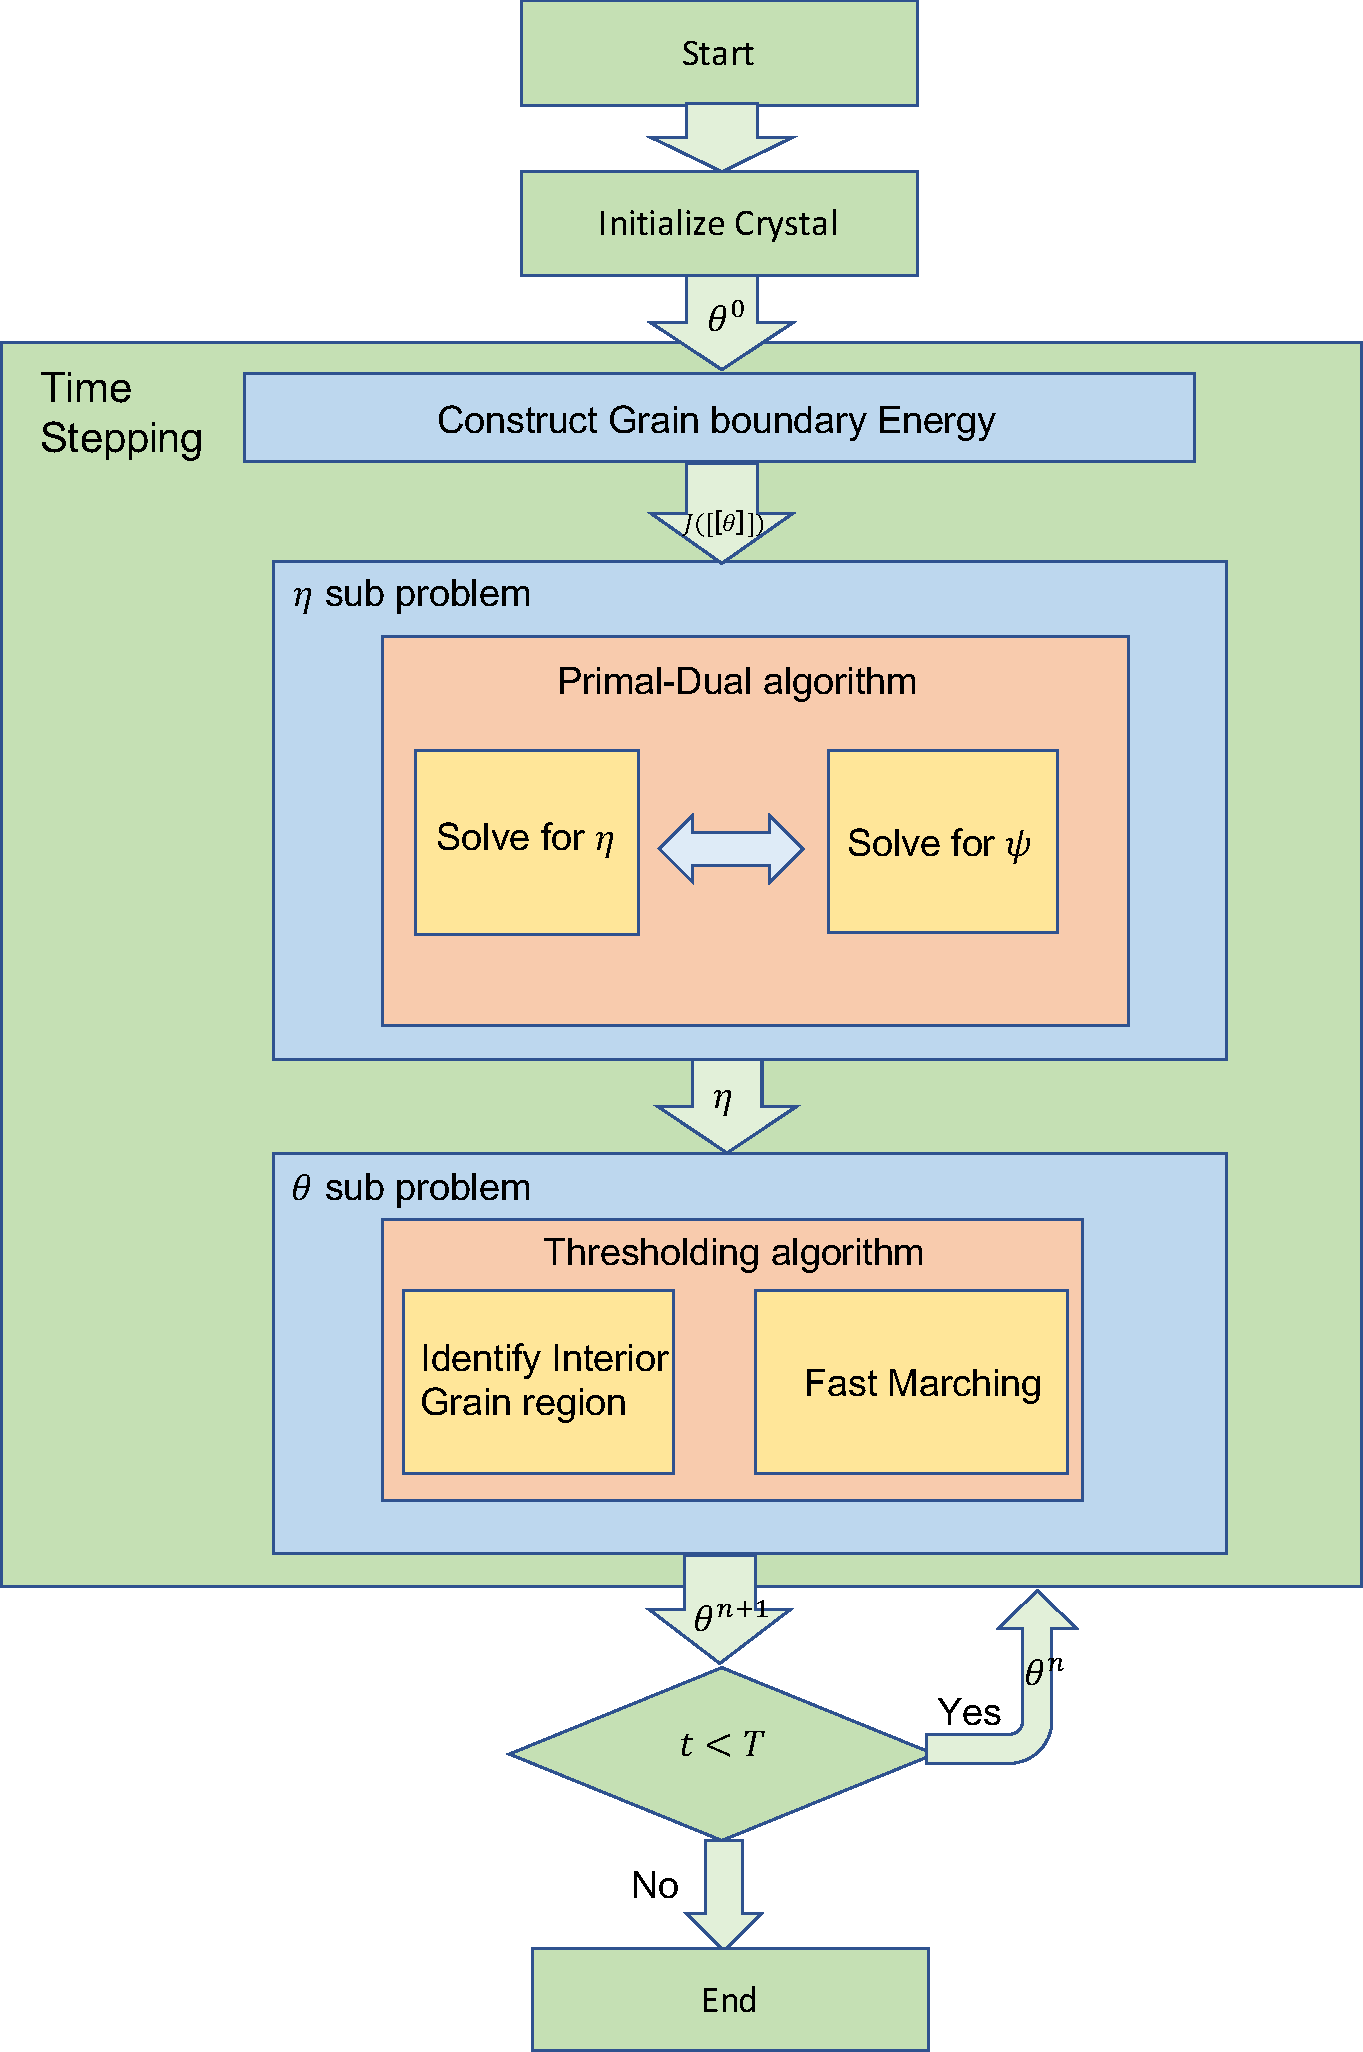
\includegraphics[width=0.7\textwidth]{Figures/flowChart.pdf}
\end{center}
\caption{Algorithm Flow chart}
\label{Fig:flow_chart}
\end{figure}
%%%%%

\section{Environment}
The current code is written by \texttt{C++} language 
and has been tested with g++ compiler. 
For Fast Fourier Transform (FFT) and inverse FFT, 
it borrows necessary operators from  \texttt{FFTW3} library. 
Simple linear algebra is operated through a \texttt{Eigen} software. 
We suggest to use a `makefile' tool to export these environment variables, 
an example format of which is as follow
\begin{tcolorbox}[colback=white]
\begin{lstlisting}[basicstyle=\footnotesize]
IDIR  += -I../../include/KWC_Simulation
IDIR  += -I../../Eigen
CC= g++
CFLAGS += -Ofast
CFLAGS += -std=c++14
CFLAGS += -lm
CFLAGS += -lfftw3_threads
CFLAGS += -lfftw3
program: 
	$(CC) KWC_driver.cpp -o main $(CFLAGS) $(IDIR)
\end{lstlisting}
\end{tcolorbox}
For data visualization, we use \texttt{ffmpeg} libraries and \texttt{Paraview}. 
Yet, those two are not mandatory.  


\section{Driver File}

We recommend to execute the program using a driver file written in \texttt{.cpp} format.
We will example basic elements of a driver file 
with an example, which runs the bicrystal simulation.
Driver files for other grain configuration can build on this basic structure. 

\subsection{Execution}

Once the driver file is successfully compiled, it will create an executable, 
Say that it is `main'. The executable can be run with following arguments, 
which stands for size of computational domain $N_x,N_y,N_z$, 
and $\epsilon$ value. 
 
\begin{tcolorbox}[colback=white]
\begin{lstlisting}[basicstyle=\footnotesize]
./main 512 512 1 0.05
\end{lstlisting}
\end{tcolorbox}

\subsection{Driver file strcuture}
\begin{itemize} \item List of required header files \end{itemize}
\begin{tcolorbox}[breakable, enhanced]
\begin{lstlisting}[basicstyle=\footnotesize]
#include <stdlib.h>
#include <math.h>
#include <string.h>
#include <time.h>
#include <float.h>
#include <stdio.h>
#include <assert.h>
#include <iostream>
#include <vector>
#include "DataOut.h"
#include "InitCrystal.h"
#include "PostProcessor.h"
#include "PrimalDual_Neumann.h"
\end{lstlisting}
\end{tcolorbox}

\begin{itemize} \item Define domain size and declare global variables \end{itemize}

\begin{tcolorbox}[breakable, enhanced]
\begin{lstlisting}[basicstyle=\footnotesize]
int main(int argc, char *argv[]){

  //Read global variables from bash
  //Define grid size and set model parameter epsilon
  int n1=atoi(argv[1]);
  int n2=atoi(argv[2]);
  int n3=atoi(argv[3]);
  double epsilon=atof(argv[4]);

  /* Construct Classes */
  int const DIM=3;
  const unsigned int lcount=1;
  int pcount = n1*n2*n3; 
  double dt= epsilon * epsilon; //initial choice of dt 
	  
  double *Xangles = new double[lcount]();
  double *Yangles = new double[lcount]();
  double *Zangles = new double[lcount]();
  double *eta = new double[pcount]();
  int *labels = new int[pcount]();
  double *energyField = new double[pcount]();
  int Nthread = 1; //The number of threads to be used for FFTW
  ...
\end{lstlisting}
\end{tcolorbox}


\begin{itemize} \item Set material types\end{itemize}

Next, we construct a material type for $\mathcal{J}$. 
You may need to set material parameters if necessary. 
\begin{tcolorbox}[breakable, enhanced]
\begin{lstlisting}[basicstyle=\footnotesize]
  //Here, 's' stands for the original KWC model of J
  char materialType='s';
  Material material;
  //set material constant value s 
  material.s=1.0;  
\end{lstlisting}
\end{tcolorbox}
Here, the material type 's' stands for simple material,
which is $\mathcal{J}$ of original KWC grain model.

\begin{itemize} \item Initialize crystal\end{itemize}

Then, we construct initialize a bicrystal. \\
\begin{tcolorbox}[breakable, enhanced]
\begin{lstlisting}[basicstyle=\footnotesize]
  //Initialize crystal: set initial condition of $\theta(x)$
  InitializeCrystal::oneD_Bicrystal_configuration(n3,n2,n1,labels);
\end{lstlisting}
\end{tcolorbox}
Other crystal configuration can be found in \texttt{InitCrystal.h} header file.
A user can also define new crystal configuration independently for one's own needs.  

\begin{itemize} \item Construct algorithm \texttt{C++} class
and link global variables \end{itemize}

\begin{tcolorbox}[breakable, enhanced]
\begin{lstlisting}[basicstyle=\footnotesize]
//Construct PD Algorithm class
double PDerror=1e-6; // tolerance of Primal-dual algorithm
int PDmaxIters=10000; // allowable iteration number of the algorithm

PrimalDual<DIM> EtaSubProblem(n3, n2, n1, PDerror, PDmaxIters,
				lcount,epsilon, Nthread);
  
//Link pointers of Global variables to the Primal-Dual algorithm class
EtaSubProblem.setUpClass(eta, Xangles, Yangles, Zangles,
labels, energyField,materialType);
  
  
\end{lstlisting}
\end{tcolorbox}

\begin{itemize} \item Run simulation \end{itemize}

\begin{tcolorbox}[breakable, enhanced]
\begin{lstlisting}[basicstyle=\footnotesize]
  //Run Primal-dual algorithm
  EtaSubProblem.run(material,epsilon);
  
  //output int type data
  DataOut::Output1Dsolution(n1, n2, 0, eta , "eta1D", n1);
  
  //Calculate Grain boundary energy and print out
  double energy = computeKWCEnergy(material.s,n1,n2,epsilon,eta,Zangles,labels);
  std::cout <<"  GB Energy:  " << energy << std::endl;
    
\end{lstlisting}
\end{tcolorbox}

\begin{itemize} \item Release memory space \end{itemize}
Once simulation is finished, we release memory spaces.
\begin{tcolorbox}[breakable, enhanced]
\begin{lstlisting}[basicstyle=\footnotesize]
  EtaSubProblem.freeMemory();	
  delete[] eta; eta=NULL;
  delete[] labels; labels=NULL;
  delete[] Xangles; Xangles=NULL;
  delete[] Yangles; Yangles=NULL;
  delete[] Zangles; Zangles=NULL;
\end{lstlisting}
\end{tcolorbox}

These are the basic structure of example files. 

In the following, we will consider other cases to
introduce other features of the code, 
e.g. how to execute the thresholding algorithm with different material type

\section{Example codes}

\subsection{KWC polycrystal simulation}

The example code \texttt{KWC\_Polycrystal.cpp} will introduce
\begin{enumerate}
\item how to set a thresholding algorithm class
\item how to generate grain evolution animation 
\end{enumerate}
The code runs the polycrystal simulation with the original KWC model. 

\begin{itemize} \item Header files \end{itemize} 
To simulate grain growth, following header files should be included
\begin{tcolorbox}[breakable, enhanced]
\begin{lstlisting}[basicstyle=\footnotesize]
#include "DataOut.h"
#include "InitCrystal.h"
#include "PostProcessor.h"
#include "PrimalDual.h"
#include "KWCThresholding.h"
\end{lstlisting}
\end{tcolorbox}

\begin{itemize}
\item Defining domain size and global variables and 
selecting the simple KWC material type\\
We skip these trivial parts, 
because they are same with the previous bicrystal simulation 
\end{itemize}

\begin{itemize} \item Initialize crystal \end{itemize} 
Now, we construct a random 2D-polycrystal
using another function define in \texttt{InitCrystal.h}
\begin{tcolorbox}[breakable, enhanced]
\begin{lstlisting}[basicstyle=\footnotesize]
//The possible maximum Z-orientation
double maxZangle = 70.0* M_PI/180.0;

InitializeCrystal::RandomCrystalConfiguration2D(n3,n2,n1,lcount,labels, 
  			   maxZangle, Xangles, Yangles,Zangles);
\end{lstlisting}
\end{tcolorbox}

\begin{itemize} \item Construct algorithm \texttt{C++} class
and link global variables \end{itemize}

The thresholding algorithm class needs an additional parameter
$\xi$ which will be used as an initial criteria to identify interior regions of grain,
i.e. if $\mathcal{J}\big( [\![ \theta ]\!] < \xi$ which  we will consider as 
grain interiors. \\

\begin{tcolorbox}[breakable, enhanced]
\begin{lstlisting}[basicstyle=\footnotesize]
double PDerror=1e-6; // tolerance of Primal-dual algorithm
int PDmaxIters=10000; // allowable iteration number of the algorithm
PrimalDual<DIM> EtaSubProblem(n3, n2, n1, PDerror, PDmaxIters,lcount,
						     epsilon, Nthread);

// Criteria for Identifying interior regions of grains
double initThresCriteria = 2*epsilon ; 

KWCThreshold<DIM> FastMarching(n3,n2,n1,lcount,initThresCriteria);

EtaSubProblem.setUpClass(eta, Xangles, Yangles, Zangles, 
			labels, energyField,materialType);
			
FastMarching.setUpProblem(eta, Xangles, Yangles, Zangles, 
			labels, energyField,'P');  
\end{lstlisting}
\end{tcolorbox}

\begin{itemize} \item (Optional) Setting FFMEPG for grain animation \end{itemize}

The developed code can generate grain evolution movie while simulation is running.
This will necessitate that \texttt{ffmpeg} is installed on the machine. 
We will convert the Z-orientation value of grains into a number between 
[0,255]. Then, we will use black-and-white images to collect pictures of grains 
at each time step. \\

\begin{tcolorbox}[breakable, enhanced]
\begin{lstlisting}[basicstyle=\footnotesize]
  
  /* movie data */
  unsigned char *pixels=new unsigned char[pcount];
  
  unsigned char *colors=new unsigned char[lcount];
  for(int l=0;l<lcount;l++){
      // Distribute colors to angles
        colors[l]=255*Zangles[l]/maxZangle;
  }
  
  char *string;
  asprintf(&string,"ffmpeg -y -f rawvideo -vcodec rawvideo -pix_fmt gray -s 
   %dx%d -r 30 -i - -f mp4 -q:v 5 -an -vcodec mpeg4 out.mp4", n1,n2);
  
  //open an output pipe
  FILE *pipeout = popen(string, "w");
  
\end{lstlisting}
\end{tcolorbox}

\begin{itemize} \item Run simulation \end{itemize}
We take 200 time steps, and the pixel grain data will be 
reformatted to black-and-white image data. \\
\begin{tcolorbox}[breakable, enhanced]
\begin{lstlisting}[basicstyle=\footnotesize]
  //Start Dynamics
  for (int i =0 ; i<200 ; i++)
  {
    PrepareFFMPEG2DPixels(n1,n2,0,pixels, labels, colors);
    fwrite(pixels, 1, pcount, pipeout);
      
    EtaSubProblem.run(material, epsilon);
    FastMarching.run(epsilon);
  }
\end{lstlisting}
\end{tcolorbox}

\begin{itemize} \item Release memory space \end{itemize}

We release memory space. In this case, we also need to take care of
the memory space used for the thresholding class. 
If one used \texttt{ffmpeg}, ones need to flush out the command 
to the shell. 
\begin{tcolorbox}[breakable, enhanced]
\begin{lstlisting}[basicstyle=\footnotesize]
  fflush(pipeout);
  pclose(pipeout);

  EtaSubProblem.freeMemory();
  FastMarching.freeMemory();
  
  delete[] eta; eta=NULL;
  delete[] labels; labels=NULL;
  delete[] Xangles; Xangles=NULL;
  delete[] Yangles; Yangles=NULL;
  delete[] Zangles; Zangles=NULL;
\end{lstlisting}
\end{tcolorbox}

\subsection{Simulation of the alternate KWC model}

The main advantage of using the alternate KWC model is
that one can freely construct the function $\mathcal{J}$ in Eq~(\ref{eqn:alternateKWC}).
In this example, we will how to use alternate simulation. 
 
\subsubsection{Design the jump function}

The example code \texttt{Design\_J.cpp} uses a Newton's iteration 
to fit $\mathcal{J}\big( [\![ \theta]\!]\big)$ to an external grain boundary energy data. 
The code takes an input file \texttt{STGB\_cu\_110.txt} which is 
the covariance model prediction of FCC [110] Symmetric-tilt-grain-boundary energy~\cite{Runnels:2016_1,Runnels:2016_2}. 
The format of the input file is as follow\\

\begin{tcolorbox}[colback=white]
\begin{lstlisting}[basicstyle=\footnotesize]
 # tiltAngle(deg)         # W_data
 # ------------            -------------  
                   0        	     0.0
                 0.5             0.10458
                   1            0.203463
                 1.5            0.296963
                   2            0.385376
                 2.5            0.468977
                   3            0.548028
                 3.5            0.598243
... (continues)
\end{lstlisting}
\end{tcolorbox}       

To construct $\mathcal{J}$, we can call \texttt{KWCDesignJ} \texttt{C++ class}.
We only need to provide the number of data and the name of input\&output file as follow.\\

\begin{tcolorbox}[breakable, enhanced]
\begin{lstlisting}[basicstyle=\footnotesize]
int main(int argc, const char * argv[]) {
     int nData=361;
     KWCDesignJ optimizer(nData,"STGB_cu_110.txt","J_cu_110.txt");
     optimizer.run(); 
     return 0;
}
\end{lstlisting}
\end{tcolorbox}


Then, the output file format, \texttt{J\_cu\_110.txt} can be later used for grain growth simulation.\\
\begin{tcolorbox}[colback=white]
\begin{lstlisting}[basicstyle=\footnotesize]
    # tiltAngle       # Jtheta # Total Energy
 # ------------  -------------   -------------
              0              0              0
            0.5      0.0432744        0.10458
              1       0.102464       0.203463
            1.5       0.171975       0.296963
              2       0.250429       0.385376
            2.5       0.337459       0.468977
              3       0.433323       0.548028
            3.5       0.502413       0.598243
... (continues)
\end{lstlisting}
\end{tcolorbox}      

\subsection{Running KWC polycrystal simulation with the designed J}

Now, we are ready to simulate grain evolution 
with crystal symmetry-invariance grain boundary energy. 
Most of program structure is same with the previous polycrystal simulation code, 
but we only need to simply replace the material type as `c' and designate 
the $\mathcal{J}$ data.\\

\begin{itemize} \item Set material types\end{itemize}

\begin{tcolorbox}[breakable, enhanced]
\begin{lstlisting}[basicstyle=\footnotesize]
char materialType='c';
  Material material;

  if(materialType =='c')  {
    material.setCovarianceModel(361, "inputs/jfun_cu_110.txt");
  }
\end{lstlisting}
\end{tcolorbox}

\bibliographystyle{unsrt}
\bibliography{references}




\end{document}
